
Para poder entender los mecanismos de la biología molecular y aprender a cómo manipularlos a favor de la ciencia, es necesario aprender como las bases de estos mecanismos funcionan. Los fundamentos de la biología molecular son pues el ADN y el dogma central de la biología, el primero siendo la base estructural de los mecanismos de genética y el segundo siendo el esquema general de lo que la biología molecular estudia mainpula.

\section{ADN: Estructura y funciones}\label{sec:ADN}

El ácido desoxirribonucléico, comunmente abreviado como ADN, es la base de la biología molecular. Es esta biomolécula la que almacena la información genética de una célula, y es también a partir del procesamiento de ella que surgen una infinidad de fenómenos de la biología. 

\marginpar{\begin{minipage}{\marginparwidth}
    \begin{figure}[H]
        \centering
        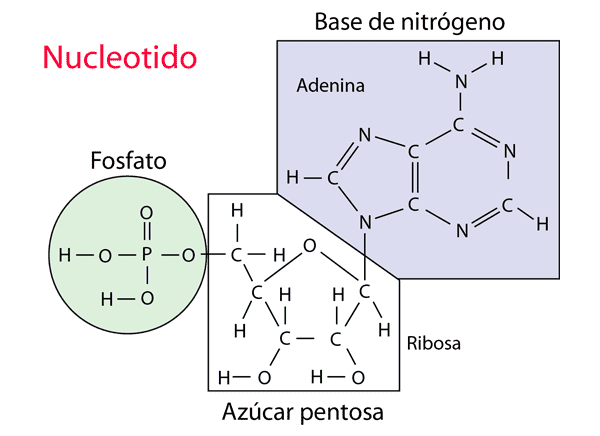
\includegraphics[width=\linewidth]{images/fig:estructura_de_un_nucleotido}
        \caption{Estructura general de un nucleótido}
        \label{fig:estructura_de_un_nucleotido}
    \end{figure}
\end{minipage}}

Al igual que el resto de biomoléculas, el ADN se compone monómeros que, unidos, forman un polímero, el ADN. Los monómeros del ADN son los nucleótidos, y estos se componen de 3 compuestos claves.

En primer lugar tenemos una base nitrogenada. Estas son compuestos orgánicos que cuentan con nitrógeno unido a ellos, y todos los organismos usan en su ADN las mismas 4 bases nitrogenadas: Adenina (A), timina (T), guanina (G) y citosina (C).

Luego de la base nitrogenada encontramos un carbohidrato, especificamente la 2-desoxi-D-ribosa, más comunmente acotada a desoxirribosa. A este carbohidrato (o azúcar) se le une una base nitrogenada en la posición 2'. 

Hasta este punto, la unión de una base nitrogenada con la ribosa se conoce como nucleósido. No es si no hasta que se une un grupo fosfato al extremo 5' del azúcar que podemos llamar a esta unión de moléculas un nucleótido, la unidad funcional del ADN.%\cite{pinillabermudezBiologiaMolecular2019}

\subsection{Niveles estructurales del ADN}

\begin{figure}[H]
    \centering
    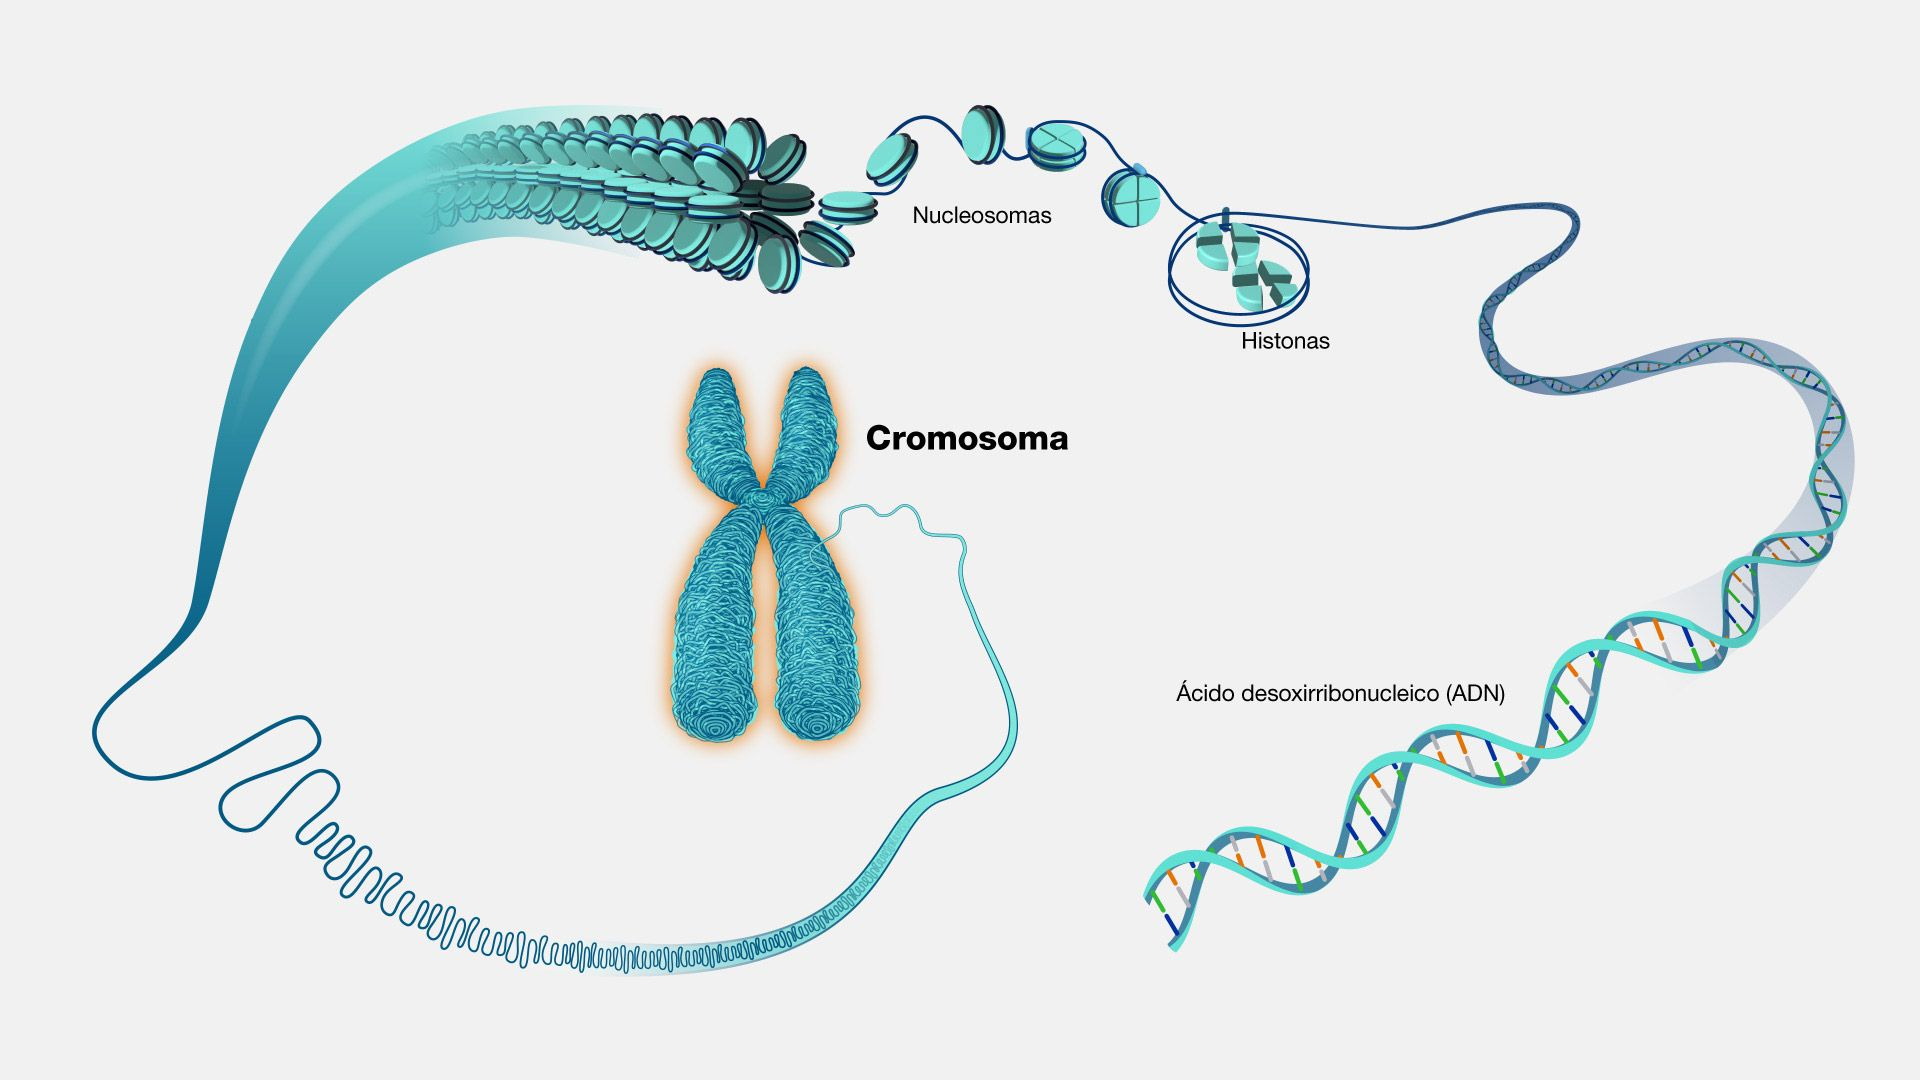
\includegraphics[width=\linewidth]{images/fig:niveles_estructurales_del_adn}
    \caption{Niveles estructurales del ADN}
    \label{fig:niveles_estructurales_del_adn}
\end{figure}

Si bien los nucleótidos son la unidad estructural del ADN, no es la mera unión de estos lo que conforma a esta biomolécula, sino que se pueden identificar varias ``etapas'', los llamados niveles estructurales, a través de las cuales se va formando el ADN, y existen cuatro niveles estructurales en el ADN.

La estructura primaria, la más básica, se compone de la secuencia de nucleótidos en una hebra de ADN. Esto se refiere pues al orden específico en que una serie de nucleótidos estén ordenados.

Como segundo estructura secundaria tendríamos a la estructura que se forma al unir dos hebras de ADN, las cuales toman una forma de doble hélice. Estas hebras tienen dos características: son complementarias y antiparalelas.

La primer característica, la complementariedad, se refiere a que las bases nitrogenadas se unen de una manera específica entre ellas. Particularmente, toda adenina (A) se une siempre a una timina (T), y toda citosina (C) se une siempre a una guanina (G). 

La otra característica, el que las hebras sean antiparalelas, describe la orientación de los diferentes extremos de las hebras, los cuales son contrarios.

El nivel terciario consta del enrrollamiento de las hebras de ADN sobre unas proteínas llamadas histonas. Este enrrollamiento hace posible que el ADN se encuentre más compacto dentro de la célula, y sirve también como mecanismo de regulación génica (\autoref{sec:acetilación}).

Estas histonas pueden crear conjuntos entre sí llamados nucleosomas.

El último nivel, la estructura cuaternaria, un conjunto de nucleosomas se agregan entre sí para formar una nueva estructura, el selenoide. Esta estructura sirve para compactar aún más el ADN en los conocidos cromosomas. Este compactamiento es de gran relevancia durante la división celular.


\subsection{Histonas y nucleosomas}

Como se mencionó anteriormente, las histonas son proteínas sobre las cuales el ADN se enrrolla para compactarse. Estas proteínas se componen de 5 partes 

Las proteínas anteriormente mencionadas, las histonas, son proteínas que enrrollan el ADN, y se componen de 5 partes:

\begin{itemize}
    \item H1: Eslabón o linker
    \item H2A, H2B, H3, H4: Core
\end{itemize}

Como igualmente se mencionó antes, los nucelosomas son a su vez conjuntos de histonas que se agrupan entre sí.



\section{Dogma central de la biología}

\begin{figure}[H]
    \centering
    \resizebox{\linewidth}{!}{\begin{tikzpicture}
\node[draw, font=\sffamily\bfseries\normalsize, inner sep=10pt] (adn) at (0,0) {ADN};
\node[draw, font=\sffamily\bfseries\normalsize, inner sep=10pt, xshift=4cm] (arn) at (adn.east) {ARN};
\node[draw, font=\sffamily\bfseries\normalsize, inner sep=10pt, xshift=4cm] (proteinas) at (arn.east) {Proteínas};

\draw[-Stealth] (adn.east) -- (arn.west) node[midway, fill=white, draw, rounded corners, font=\sffamily\scriptsize] {Transcripción};
\draw[-Stealth] (arn.east) -- (proteinas.west) node[midway, fill=white, draw, rounded corners, font=\sffamily\scriptsize] {Traducción};

\node[draw, rounded corners, font=\sffamily\tiny, xshift=0.5cm, yshift=1cm] (replicacion adn) at (adn.east) {Replicación del ADN};
\draw[-Stealth] (adn.east) to[out=0, in=-90] (replicacion adn) to[out=180, in=90] (adn.north);

\node[draw, dashed, rounded corners, font=\sffamily\tiny, xshift=0.5cm, yshift=1cm] (replicacion arn) at (arn.east) {Replicación del ARN};
\draw[-Stealth, dashed, color=gray] (arn.east) to[out=0, in=-90] (replicacion arn) to[out=180, in=90] (arn.north);

\node[draw, rounded corners, font=\sffamily\tiny, xshift=1.5cm, yshift=-1.25cm, text width=1.5cm, align=center] (transcripcion_inversa) at (adn.east) {Transcripción inversa};
\draw (arn.south) to[out=-90, in=0] (transcripcion_inversa.east);
\draw[-Stealth] (transcripcion_inversa.west) to[out=180, in=-90] (adn.south);

\node[draw, dashed, rounded corners, align=center, text width=2.25cm, font=\sffamily\tiny, xshift=-1cm, yshift=-1.75cm] (drts) at (proteinas.west) {Transcriptasa inversa asociada a defensa (DRTs)};
\coordinate (drts checkpoint) at ([xshift=-5cm]drts.west);
\draw[-Stealth, dashed, color=gray] (proteinas.south) to[out=-90, in=0] (drts) to[out=180, in=0] (drts checkpoint) to[out=180, in=-90] (adn.south);
\end{tikzpicture}}
    \rule{\linewidth}{0.2pt}
    \caption{Dogma central de la biología}
    \label{fig:dogma_central}
\end{figure}

El dogma central es el esquema general de como funciona la biología molecular. Nos describe los pasos generales que toma la información genética para generar los diferentes productos de esta, y el conocerlo a fondo nos permite manipularlo para obtener cosas como compuestos de interés.

El dogma central describe 3 procesos principales: la replicación del ADN, la transcripción de este a ARN, y la traducción del ARN a proteínas.  